%!TEX root = ../thesis.tex

\section{実験概要}
本章では, 前章の実験で使用した教師データに問題があるか調査を行う. 具体的には, 5章で最も成功率の高かった実験(以後, 実験1と呼ぶ)で使用した教師データと, 前章の実験(以後, 実験2と呼ぶ)で使用した教師データを入れ替えて学習を行う. これにより, 目標角速度とカメラ画像のどちらに問題があるか判明するのではないかと考える. 

\section{実験方法}
原因の調査を行うために, シミュレータを用いた実験を行う. 実験環境, 実験装置は前章と同様のシミュレータ環境を用いる.また, 学習器の訓練条件, 学習したモデルを用いたテストなどの条件は前章と同様とする. 実験1の目標角速度と実験2のカメラ画像の組み合わせを実験3, 実験1のカメラ画像と実験2の目標角速度の組み合わせを実験4とする

\newpage
\subsection{実験結果と考察}
実験結果を\ref{tb:inves}に示す. 分母の10は実験回数を示しており, 分子の数は成功回数を示している. 結果的に, 実験3の成功回数は30回中0回, 実験4の成功回数も30回中0回となった. 失敗した箇所も, 概ね実験2と同様に, 直進時に目標経路から外れて, 壁に衝突して失敗した. このことから, カメラ画像から左右に切り抜く方法では, ロボットをヨー方向に±5[deg]回転させた際の画像を再現できていないと考えられる. また, 目標角速度に関しても, 実験1ではそれぞれの位置と角度でルールベース制御器の出力を取得してしたいた. しかし, 実験2ではロボットを走行させながら収集した角速度にオフセットを加えることで, 各位置と向きを考慮した目標角速度を生成している. この方法では, 経路追従を継続するのに必要な目標角速度を再現できていないと考えられる. オフセットの値に関しても, 実験1の結果を基に値を決めたが, この値も適切ではない可能性がある. 

\begin{table}[h]
  \centering
  \caption{Number of successes in the experiments of simulator}
  \begin{tabular}{|c|c|} \hline
      Experiments & Number of successes \\ \hline
      Exp. 3 & 0/30 \\ \hline
      Exp. 4 & 0/30 \\ \hline
    \end{tabular}
  \label{tb:inves}
\end{table}

% 前章で最も成功率の高かった際の教師データを実験1, 本章の教師データを実験2として比較を行う. これにより, 目標角速度とカメラ画像に問題があるかを調査する. \figref{Fig:ratio}に目標角速度の割合を比較したグラフを示す. 

% \begin{figure}[h]
%   \centering
%   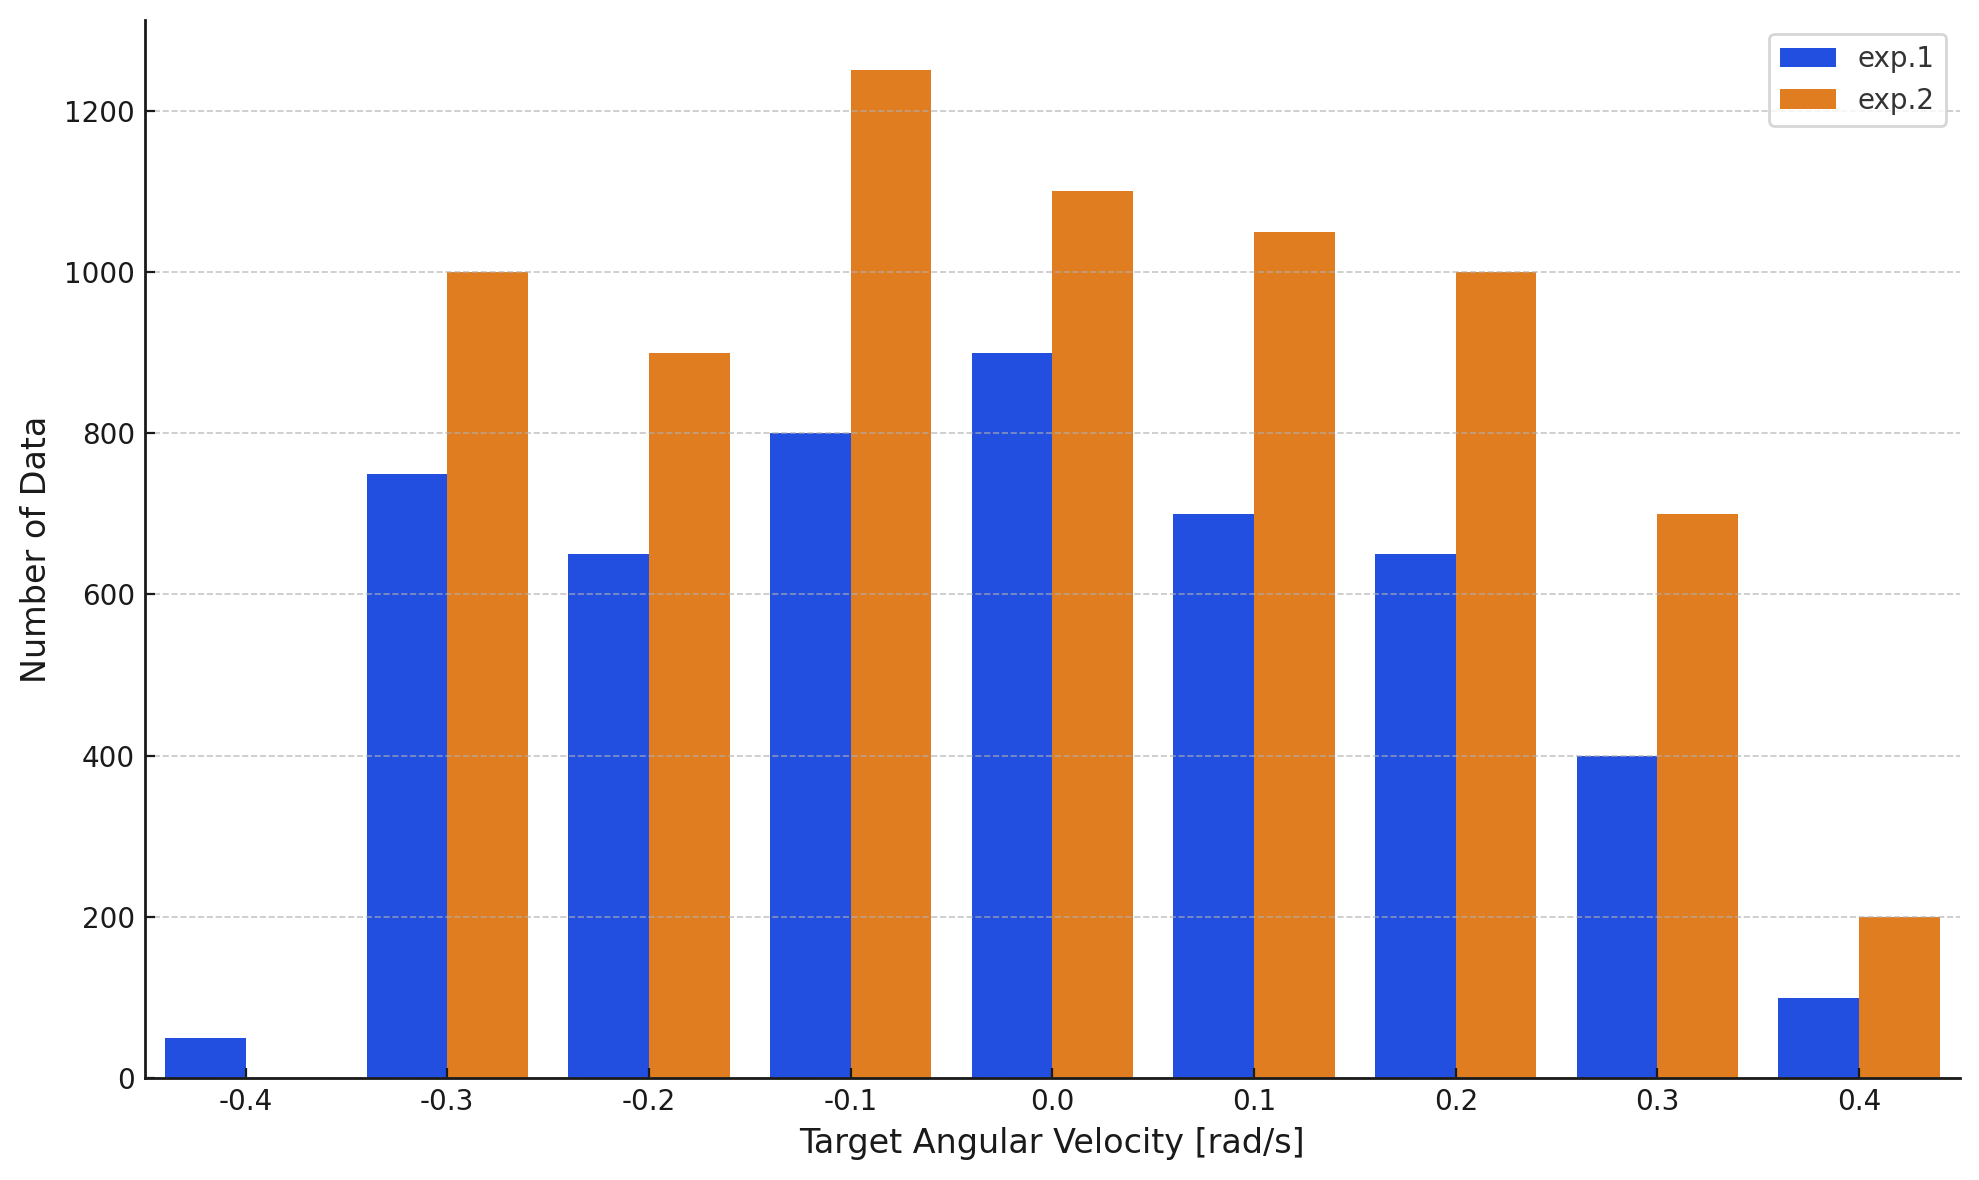
\includegraphics[keepaspectratio, scale=0.5]{images/output.png}
%   \caption{Comparison of target angular velocity ratios}
%   \label{Fig:ratio}
% \end{figure}

% 実験1と実験2の教師データを入れ替えて実験を行った. まず, 実験1のカメラ画像と実験2の目標角速度の組み合わせで学習を行った.